\subsection{Physical SPX dynamics and the volatility risk premium}
\label{sec:spx-physical-premium}
% [AI-DRAFT BEGIN: dated SPX physical-to-pricing exercise. Author pass pending.]
We estimated the latent spot-volatility dynamics under $P$ using 5,738 SPX
log returns and VIX closes from 22 September 2003 to 14 July 2026.
On 4,153 of those sessions we also observed Oxford--Man five-minute realised
variance, distributed with the \texttt{rumidas} package.\footnote{\url{https://cran.r-universe.dev/rumidas/doc/page/rv5}.}
That series ends on 31 March 2020. Subsequent filter updates use returns and VIX alone.

We applied an approximate Gaussian filter to $x_t=\log\sigma_t$ on a $1/252$-year session grid.
We subtract the historical sample mean from each return to measure the common Brownian
shock. Log intraday realised variance has measurement equation
$\log \mathrm{RV}_t=2x_{t-1}+\log(1/252)+a_R+u_t$, with an estimated offset and noise scale.
For VIX in decimal units we used $\log I_t=\log F^{Q_h}_{30/365}(\sigma_t)+e_t$, with $F$
from~\eqref{eq:index-map}. We estimated the two noise scales and a constant historical
pricing coefficient $C_{Q,h}$ together with the physical coefficients by quasi-likelihood.
We computed the VIX map on a log-volatility grid and gave each session equal weight.

The physical estimates are $(\theta_P,\kappa_{1,P},\kappa_{2,P},v)=
(0.1793,5.615,11.133,1.562)$, with
$\beta=-1.310$, $\varepsilon=0.851$ and $\rho=-0.839$.
Fixing $\kappa_{1,P}=1$ and re-estimating the other coefficients lowers the mean
daily quasi-log-score by 0.039.
The fitted log-measurement standard deviations are 0.640 for RV and
0.010 for VIX. The historical VIX fit reaches the admissible boundary
$C_{Q,h}=0$. At fixed physical coefficients and spot, this boundary gives the
highest 30-day model VIX in the admissible family.
The filtered median of spot volatility on 14 July is 13.96\%.

For the 15 July SPXW quotes, \eqref{eq:pq-map} fixes $A=1.007$, $B=-3.619$
and the two diffusion loadings. We fit only $\delta=C_Q-C_P=\beta\ell_0+\varepsilon\ell_1$.
First we update the historical filter with the 15 July return and VIX close, keeping
the historical coefficients fixed. Holding that closing state at
13.06\%, the option fit gives $\delta=-2.017$
and $(\theta_Q,\kappa_{1,Q},\kappa_{2,Q})=(0.1886,
5.338,9.116)$.
The resulting 30-day model VIX is 14.88 points.
Second, we require each candidate $C_Q$ to reproduce the observed VIX close of
15.67 points by inversion for $\sigma_0$.
This gives $\delta=-2.064$ and pricing parameters
$(\theta_Q,\kappa_{1,Q},\kappa_{2,Q})=(0.1889,
5.332,9.070)$.
In both fits the negative premium reduces $C_Q=\kappa_{2,Q}$ and raises the volatility
drift at each positive state. The two Brownian risk prices require additional information
to separate them. The return equation here estimates innovations and leaves the
equity risk premium unspecified.

\begin{table}[htbp]\centering\small
\begin{tabular}{@{}lrrrrrrrr@{}}\toprule
 & Option & & \multicolumn{5}{c}{IV RMSE (percentage points)} & Inside\\
\cmidrule(lr){4-8}
Specification & params. & $\sigma_0$ & Pooled & 12d & 30d & 65d & 93d & (\%)\\\midrule
Premium, filtered spot & 1 & 0.1306 & 2.431 & 3.708 & 2.287 & 1.606 & 1.443 & 2.9 \\
Premium, VIX inversion & 1 & 0.1404 & 2.599 & 3.964 & 2.354 & 1.762 & 1.629 & 1.9 \\
Premium and spot & 2 & 0.1231 & 2.401 & 3.637 & 2.316 & 1.548 & 1.437 & 3.9 \\
Free drift and spot & 4 & 0.1294 & 2.096 & 3.525 & 1.978 & 0.859 & 0.705 & 5.8 \\
Unrestricted & 6 & 0.0722 & 0.447 & 0.662 & 0.463 & 0.137 & 0.357 & 20.4 \\
\bottomrule\end{tabular}
\caption{Historical restrictions on the 15 July 2026 SPXW fit. All rows use the same
103 midpoint IVs, four equally weighted maturities and full-state PDE.
The inside-spread percentage counts quotes equally.}
\label{tab:spx-physical-premium}\end{table}

The largest discrepancy in Table~\ref{tab:spx-physical-premium} occurs at 12 days.
At the strike nearest the forward the VIX-inverted fit gives 14.5\%
IV against a midpoint of 10.0\%. At log-moneyness
-15.0\% it gives 22.9\% against
31.6\%. Figure~\ref{fig:spx-physical-smiles} shows how this
discrepancy varies by strike. Allowing the options to set $\sigma_0$ freely changes
pooled RMSE from 2.599 to 2.401 percentage points.
The resulting model VIX is 14.48 points.
Freeing all three pricing drift coefficients with the historical loadings gives
an RMSE of 2.096. The fitted $\kappa_{1,Q}$ is at the lower search
bound of 0.05. The unrestricted fit gives
0.447 at the upper $\kappa_{1,Q}$ bound of
30,
with $(\beta,\varepsilon)=(-4.176,
4.724)$. A change of equivalent measure preserves
both diffusion loadings, so the historical model cannot generate this pair by a drift change.
These are in-sample pricing errors on one surface. The historical estimates depend on the
single-factor specification and the approximation of market VIX by the variance-swap map.

\begin{figure}[htbp]\centering
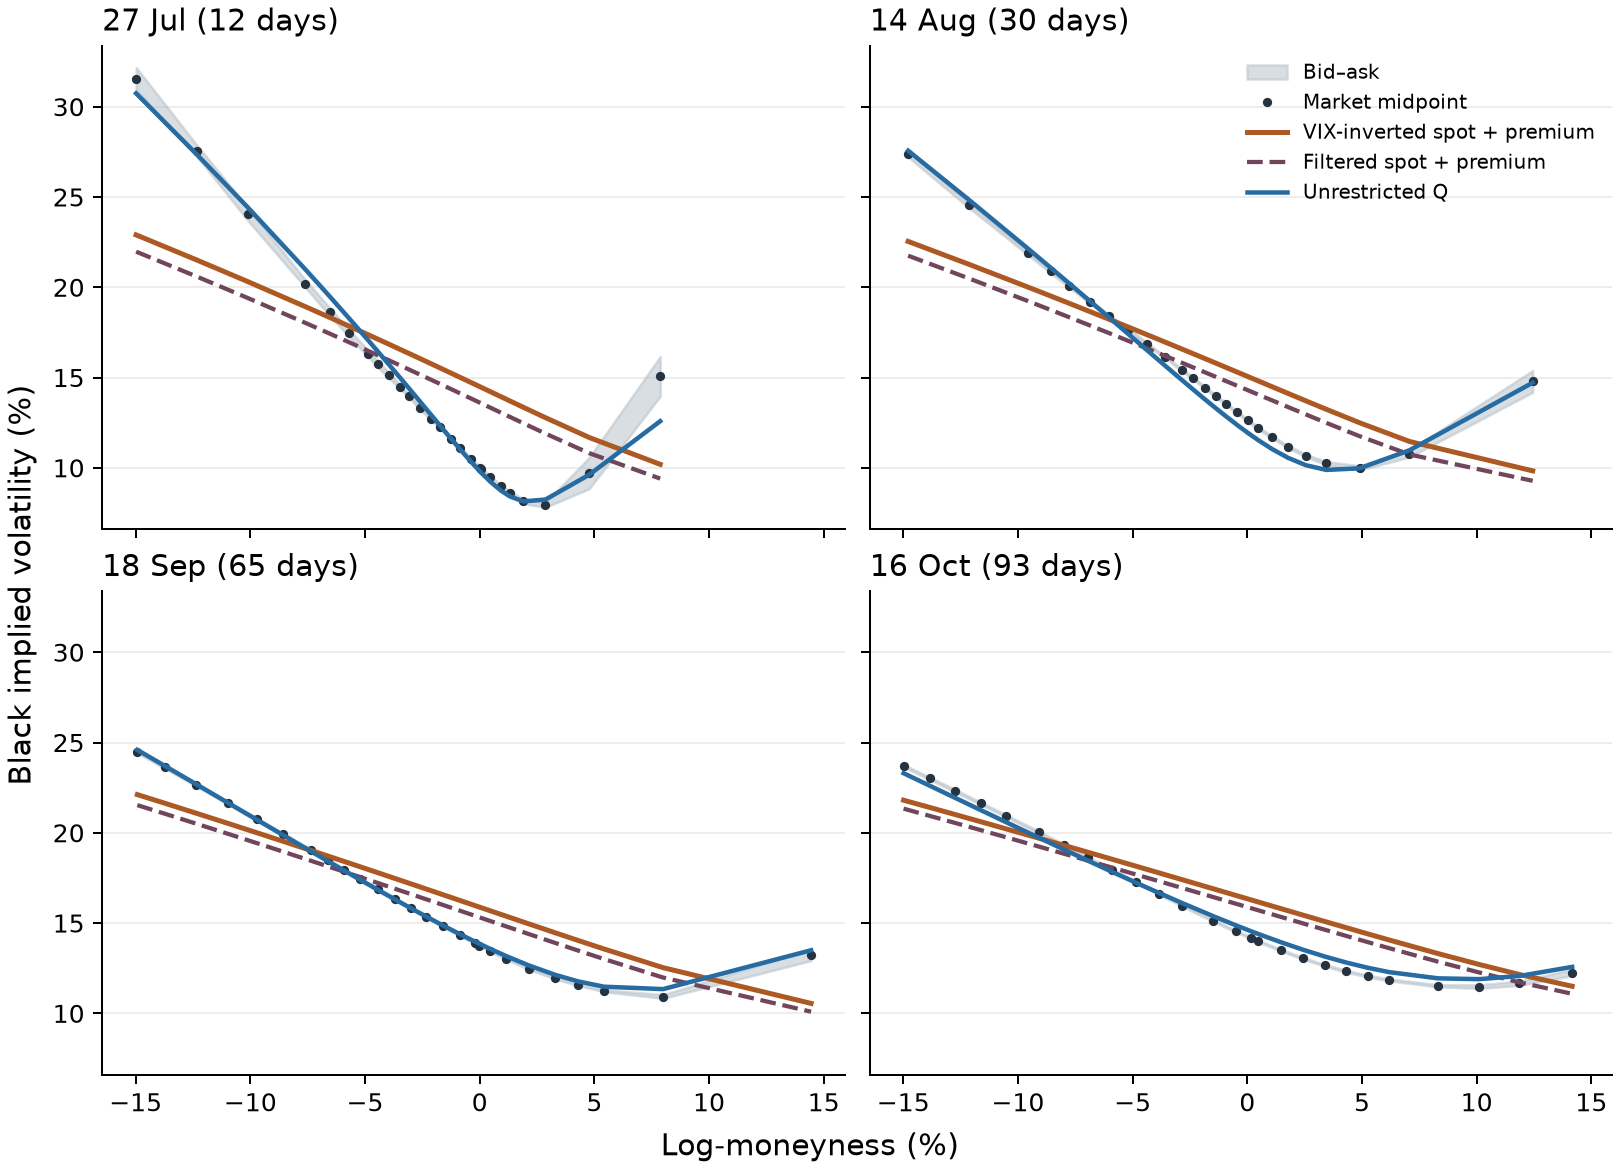
\includegraphics[width=0.90\linewidth]{figures/spx_physical_pricing_20261124/spx_smiles.png}
\caption{SPXW implied volatilities on 15 July 2026. The two historically restricted
fits use the filtered spot (dashed) or the VIX-inverted spot (orange). The blue line gives
the unrestricted pricing fit. Points and shading show quote midpoints and bid--ask intervals.}
\label{fig:spx-physical-smiles}\end{figure}
% [AI-DRAFT END]
